%Når du starter på en opgave skriver du \begin{opgave}{navnet på opgaven}{sværhedsgrad}, hvor sværhedsgraden skrives som 1,2 eller 3, hvor 3 er den sværeste. 
%Når opgaven er slut skrives \end{opgave}. 
%Såfremt der er delopgaver skrives delopgaver som \opg 

%Eksempel på opgave 
%\begin{opgave}{Polære koordinater}{1}
%  Den kinetiske energi af et legeme, der bevæger sig i 2D-planet er
%  i kartesiske koordinater ($x$ og $y$) givet ved ligning
%  (1.11).\\  
%  \opg Beregn $\dt{x}$ og $\dt{y}$ i polære koordinater og vis
%  derefter, at den kinetiske energi udtrykt i polære koordinater er
%  givet ved ligning (1.12).
%\end{opgave}
\chapter{Astrofysikopgaver}
\section*{Astrofysik}
\begin{opgave}{Rødforskydning af kvasar}{1}
	Kvasarer (eng:”quasars” fra ”quasi-stellar radio sources”) er de mest energirige og
	fjerne medlemmer af objekterne kendt som aktive galaksekerner (eng:”AGN: Active
	Galactic Nuclei”). Kvasarer har siden deres opdagelse været omgivet af mystik, men
	der er nu opnået generel enighed om, at de er kompakte regioner i massive galakser,
	der indeholder det centrale supermassive sorte hul. De kæmpe mængder energi der
	bliver udstrålet af kvasarerne stammer fra al stoffet, som falder ind mod det sorte
	hul og bliver slynget ud.
	Et kvasar-spektrum er vist i Figur \ref{kvasar}.
	\\
	I Balmer-serien hopper en elektron til 2. orbital fra en mere exciteret tilstand. Den første af disse kaldes H-$\alpha$ og er faldet fra orbital 3 til 2. Den næste er H-$\beta$ fra orbital 4 til 2 osv. Fotoner, der udsendes ved H-$\alpha$-overgangen, har en bølgelængde på 656 nm. Ofte måler man i ångstrøm (Å) som er $10^{-10}$ m.\\
	%Aflæs bølgelængden for H-$\beta$ på Figur \ref{spektrum} og beregn rødforskydningen.
	\begin{figure}[h!]
		\centering
		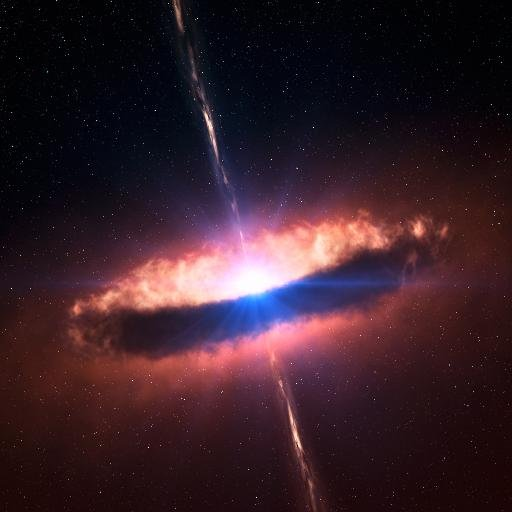
\includegraphics[width=0.3\textwidth]{Astrofysik/Astrofig/kvasarkunst.jpg}
		\caption{En kunstnerisk forestilling af en kvasar.} %https://pbs.twimg.com/profile_images/683524276058763264/xyAc-NvD.jpg
		\label{kvasarkunst}
	\end{figure}
	\begin{figure}[h!]
		\centering
		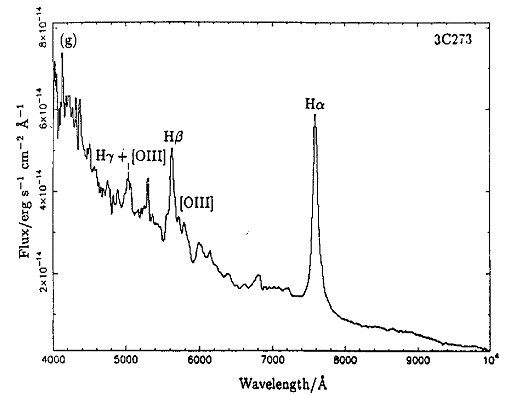
\includegraphics[width=0.5\textwidth]{Astrofysik/Astrofig/kvasar.png}
		\caption{ } %http://www.astrosurf.com/buil/us/spe6/qso1.gif
		\label{kvasar}
	\end{figure}
	\opg Ud fra din viden om H-$\alpha$-overgangen, bevæger kvasaren sig så mod eller væk fra os?
	\opg Hvad er kvasarens radielle hastighed?
	\opg Man ser tit, at spektrallinjerne fra kvasarer er meget brede, fordi gassen bevæger sig hurtigt omkring det sorte hul, hvilket giver en Doppler-forbredning
	(lyset bliver både rød- og blåforskudt). Estimér bredden af H-$\alpha$-linjen, $\Delta\lambda_{obs}$, og udregn gassens fart ved 
	\begin{align}
	v_{gas}=\frac{\Delta \lambda_{obs}}{2\lambda_{0}}c
	\end{align}
	Mål ca. halvvejs oppe, det behøver ikke være så præcist.
\end{opgave}
\begin{opgave}{Dopplerforskydning}{2}
	Formlen for frekvensen ved Dopplerforskydning er
	\begin{align}
		f_{obs} = \frac{c+v_{obs}}{c+v_{kilde}} f_{kilde},
	\end{align}
	hvor $c$ er lydens hastighed i mediet, $f_{obs}$ er den observerede frekvens (udefra), $f_{kilde}$ er den udsendte frekvens, $v_{obs}$ er observatørens hastighed og $v_{kilde}$ er kildens hastighed.
	\opg En politibil kører mod dig 30 meter væk, men er 20 meter fra centrum af vejen når du kigger ligeud (se skitsen på Figur \ref{politi}). Tegn hastighedsvektoren og hastighedskomponenterne der peger henholdsvis parallelt med din synsvinkel og vinkelret på den. Tænk over om den radielle hastighed er positiv eller negativ.
	\opg Bilens speedometer viser, at den kører 50 km/t. Brug trigonometri til at beregne hvor stor en hastighedskomponent, der peger mod dig (radiel hastighed). %Skitsér groft en graf over radiel hastighed som funktion af tid og antag, at bilens hastighed er konstant.
	\opg Politibilens sirene udsender lyd med en frekvens på 800 Hz. Du står stille, og det er en let kølig dag med 15 grader, hvor lydens fart i luft er 340 m/s. Ved hvilken frekvens hører du tonen?
	\begin{figure}[h!]
		\centering
		\includegraphics[width=0.5\textwidth]{Astrofysik/Astrofig/politi.png}
		\caption{ }
		\label{politi}
	\end{figure}
\end{opgave}
\begin{opgave}{Galaksen M87 i Virgohoben}{1}
	Galaksen M87 ligger i centrum af den nærmeste store
	galaksehob Virgohoben. Rødforskydningen af lys fra M87 og dermed fra centrum af
	Virgohoben er målt til $z = 0.00436$. Vi antager en Hubblekonstant på $H_0 = \SI{70}{\kilo\metre\per\second\per\mega\parsec}$.
	\opg Beregn afstanden til M87. Gør rede for dine antagelser. \\
	
	På vores teleskoper på Jorden modtager vi en samlet flux fra M87 på $f_\text{M87} = \SI{3.68e-12}{\watt\per\metre\squared}$.
	\opg Brug den information til at give et estimat over det totale antal stjerner i M87, idet vi
	antager, at de alle har samme luminositet som Solen, $L_\odot=\SI{3,839e26}{\watt}$.
\end{opgave}
\begin{opgave}{Afstandsbedømmelse i nabolaget}{2}
	En stjerne har en tilsyneladende magnitude på 17,5 og en absolut magnitude på -1,27.
	\opg Hvad er afstanden til stjernen? \\
	
	Hvis lysmængden fra et himmellegeme reduceres undervejs mod jorden, vil det se ud til at være længere væk, end det faktisk er. Det ses ved at den observerede flux mindskes, og den tilsyneladende magnitude stiger. Der gælder her at
	\begin{align*}
	m_{faktisk}-m_{obs} = -2,5 \log \left( \frac{f_{faktisk}}{f_{obs}} \right)
	\end{align*}
	\opg Det oplyses nu, at lyset på sin vej fra stjernen til os er blevet reduceret med 60\% pga. udslukning fra interstellart støv. Hvad er den faktiske afstand til stjernen?
\end{opgave}

\begin{opgave}{Afstande}{2}
	\\  
	\opg Opskriv luminositetsafstanden $D_L$ som funktion af vinkelafstanden $D_A$.
	\opg I et fladt univers er $D_M=D_C$. $D_C$ kaldes comoving distance, og med $\Omega_m=0.3$ og $\Omega_{\Lambda}=0.7$ opfører det sig som plottet på Figur \ref{comoving}. 
	Hvor stor er $D_L$ og $D_A$ ved $z=1$? \\
	Hvad med ved $z=9$? Giver ændringerne mening?
		\begin{figure}[h!]
			\centering
			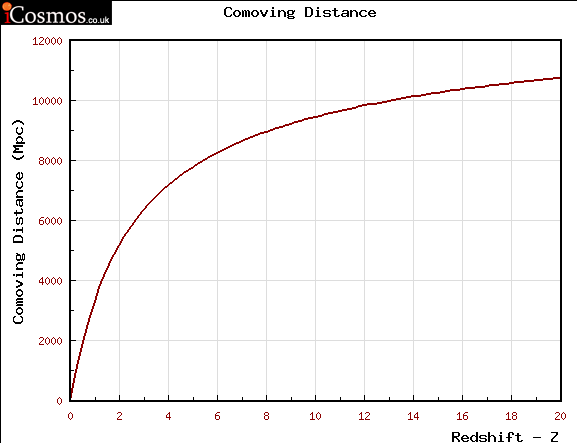
\includegraphics[width=0.5\textwidth]{Astrofysik/Astrofig/ComovingDistance.png}
			\caption{ } %http://www.icosmos.co.uk/index.html
			\label{comoving} 
		\end{figure}
	\opg Hvor stor er den radielle hastighed for et objekt med $z=10$? Oplys svaret som procent af lysets fart i vakuum. Dengang var universet for resten kun  478 mio. år gammelt.
\end{opgave}

\begin{opgave}{Himmellegemers overfladetemperatur}{3}
	Når et himmellegeme modtager stråling fra en nærliggende stjerne, vil noget af denne stråling reflekteres, og det bidrager derfor ikke til opvarmning af planeten. Albedoen $A$ er et tal fra 0 til 1 som angiver andelen af lyset, der reflekteres fra et objekt. 1 angiver 100 \% reflektion og derved at intet lys absorberes.
	\opg Vis først, at en planet eller måne med
	radius $R_m$ i en afstand $d$ (som luminositetsafstand) fra Solen og med en albedo-værdi på
	$A$ vil absorbere energien
	\begin{equation}
	L_\text{abs} = \frac{R_\odot^2\sigma T_\odot^4 \pi R_m^2}{d^2} \left( 1 - A \right),
	\end{equation}
	hvor $R_\odot$ og $T_\odot$ er hhv. radius og temperatur af Solen. \emph{Hint: man kan sige, at den del af planeten eller månen der er vendt mod Solen udgør et areal givet ved $\pi R_m^2$.} 
	\opg Hvis en måne eller planet roterer hurtigt, udsender den energi givet ved luminositeten $L_\text{uds}$ i ligning 1.25 i kompendiet. Solen er en stjerne i termisk ligevægt, så vi kan derfor skrive $L_\text{abs}=L_\text{uds}$. Vis, at temperaturen på overfladen af en planet eller måne, $T_m$, kan udtrykkes som
	\begin{equation}
	T_m = T_\odot \left( \frac{1-A}{4} \right)^{1/4} \left(\frac{R_\odot}{d} \right)^{1/2}
	\end{equation}
	\emph{Hint: start med at sætte $L_\text{abs}=L_\text{uds}$.} 
	\opg Saturns måne Mimas er placeret i en elliptisk bane omkring Saturn og  massen af Mimas er $M_\text{Mimas} = \SI{3,751e19}{\kilo\gram}$. Derudover er månens albedo $A_{Mimas} = 0,962$, mens Solens overfladetemperatur er $T_\odot = \SI{5778}{\kelvin}$, Solens radius er $R_\odot = \SI{6,955e5}{\kilo\metre}$, og middelafstanden mellem Mimas og Solen er $d_{\text{Mimas}} = \SI{1,43e9}{\kilo\metre}$. \\
	Beregn ud fra oplysningerne en teoretisk temperatur på overfladen af Mimas. Gøre rede for dine antagelser.
	\opg Cassini-rumsonden vurderede temperaturen på overfladen af Mimas til at være ca. \SI{65}{\kelvin} - hvad kan forskellen mellem den teoretiske og den observede temperatur skyldes?
\end{opgave}
\begin{opgave}{Skalafaktor}{1}
	Temperaturen af den kosmiske mikrobølgebaggrund er i dag 2.73 K. Strålingen blev udsendt ved "rekombinationen", hvor universet var koldt nok til at elektroner kunne binde sig til atomerne. Det var en mindre exciteret tilstand, så atomerne udsendte energi som fotoner. Man kan måle, at det har krævet en temperatur på maks 3000 K. Brug at temperaturen udviklede sig som
	\begin{align}
		T(t)=\frac{T_0}{a(t)}
	\end{align}
	til at finde ud af, ved hvilken rødforskydning rekombinationen fandt sted.
\end{opgave}

\begin{opgave}{Fladt univers med stof}{3}
	Forestil dig et fladt univers kun med stof.
	\opg Opskriv densitetsparametrene.
	\opg Opskriv skalafaktoren som funktion af tid.
	\opg Du står i nutiden $t_0 = 13,8$ mia. år og kigger på himlen. For en galakse med $z=1$, hvor længe skal du så observere den før rødforskydningen ændres med en $10^6$.-del? %Antag Hubblekonstanten er $H_0=70 km s^{-1} Mpc^{-1}$.
\end{opgave}

\begin{opgave}{Kosmologiske parametre}{3}
	%\opg Antag universet kun består af én komponent og er fladt. Hvordan afhænger denne komponents densitet af tiden? (Find $\rho(t)$) 
	\opg Opskriv Friedmannligningen, hvor du indsætter densiteterne af de forskellige komponenter. Se bort fra $\frac{\Lambda}{3}$-leddet, nu hvor du inkluderer densiteten af kosmologisk konstant i stedet.\\
	Hvad er $H^2$ som funktion af de nuværende værdier af parametrene?
	\opg Betragt nu vores univers, der er fladt. Hvornår bestod universet 50 \% af stråling og 50 \% stof? Mørk energi var der så lidt af, at det kunne negliceres dengang. Antag at skalafaktoren kun udvikler sig baseret på mængden af stråling og at universets nuværende alder er $13,8$ mia. år.
	\opg I virkeligheden sluttede den strålingsdominerede periode 47.000 år efter big bang. Hvorfor giver forrige delopgave noget andet?
	\opg Hvor meget kosmologisk konstant $\rho_\Lambda$ var der dengang? %Hvor stor en del af universet var kosmologisk konstant dengang?
\end{opgave}
\begin{opgave}{Andromeda-galaksen}{1}
	\begin{figure}[h!]
		\centering
		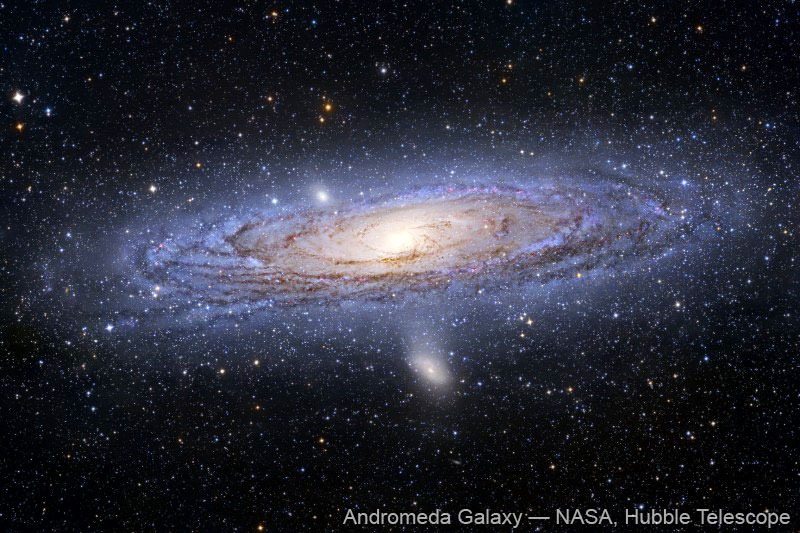
\includegraphics[width=0.5\textwidth]{Astrofysik/Astrofig/andromeda.jpg}
		\caption{  } %https://upload.wikimedia.org/wikipedia/commons/9/98/Andromeda_Galaxy_%28with_h-alpha%29.jpg
		\label{andromeda} 
	\end{figure}
	Andromeda-galaksen eller Messier-31 (M31) er den nærmeste spiralgalakse, og den største galakse i den Lokale Gruppe, som er en samling af ca. 50 galakser, heriblandt vores egen, Mælkevejen.  
	\opg Ligesom Mælkevejen er Andromedagalaksen en spiralgalakse, hvor alting kan antages at bevæge sig
	rundt om centrum i en cirkelbevægelse. Fra målinger på galaksen vurderes
	rotationshastigheden $v_{rot}(r)$ at vokse i de inderste få \SI{}{\kilo\parsec} fra centrum, hvorefter den flader ud
	og bliver konstant $v_{rot}(r) = v_{rot,max}$. Det vurderes, at $v_{rot,max} = \SI{230}{\kilo\metre\per\second}$. \\
	Giv et estimat af massen af Andromedagalaksen inden for radius $R = \SI{100}{\kilo\parsec}$ i enheder af Solens masse $M_\odot = \SI{1.9891e30}{\kilo\gram}$.
	\opg Det observerede lys fra Andromeda har en rødforskyning på $z = -0.001$.
	%\opg Det observerede lys fra Andromeda har en rødforskydning på $z = −0.001$.
	Hvad er Hubbleafstanden til galaksen, fundet ved hjælp af Hubbles lov? Antag Hubblekonstanten er $H_0=70 \text{km s}^{-1} \text{Mpc}^{-1}$.
	\opg Gennem andre metoder har man fundet afstanden til 2,5 mio. lysår. Hvornår støder Andromeda og Mælkevejen sammen? Hvad tror du, det kommer til at betyde? Antag hastigheden er konstant, og Andromeda har direkte kurs mod os.
\end{opgave}

\begin{opgave}{Betelgeuse}{1}
	Betelgeuse er en af de mest lysstærke stjerner på nattehimlen og findes i stjernebilledet Orion. Radius af Betelgeuse er målt til 1200
	gange Solens radius, $R_\odot=\SI{6,958e5}{\metre}$, med en overfladetemperatur på $T_B=\SI{3300}{\kelvin}$, mens Solens overfladetemperatur er $T_\odot=\SI{5778}{\kelvin}$. 
	\opg Bestem Solens og Betelgeuses luminositet i enheden \SI{}{\watt}, og enheder af Solens luminositet i tilfældet Betelgeuse.
	\opg Afstanden fra jorden til Betelgeuse er $d_B=\SI{642,5}{\lightyear}$. Bestem fluxen på jorden fra Betelgeuse og gør rede for nødvendige antagelser.
	\opg Afstanden fra jorden til Solen er $d_\odot=\SI{1}{AU}$. Hvor langt fra Betelgeuse er fluxen den samme, som fluxen fra solen er på jorden?
	\opg Voyager 1 satelitten er i dag $d_V=\SI{139}{AU}$ fra Solen og den stjerne, som er nærmest jorden, Proxima Centauri, befinder sig i afstanden $d_{PC}=\SI{4,3}{\lightyear}$. Hvordan er afstanden fra før sammenlignet med disse?
\end{opgave}

\begin{opgave}{Massen af Solsystemet}{1}
	Planeten Neptun, Solsystemets yderste planet, bevæger sig i en bane, der kan antages cirkulær, med  en baneradius på $R=\SI{30}{AU}$ og en periode på $P=\SI{164,8}{yr}$.
	\opg Bestem Neptuns gennemsnitlige banefart idet perioden er tiden det tager at gennemløbe cirkelbanen.
	\opg Estimer den totale masse af solsystemet og sammenlign med Solens masse.
\end{opgave}
%\begin{opgave}{Mere filosofiske spørgsmål}{1}
%	\opg Mange parametre og konstanter i universet har akkurat værdier, der tillader os at eksistere. Det fremkommer usandsynligt bare at have et univers, der ikke går under på et splitsekund og indeholder stabil masse. Hvor mange mulige forklaringer kan du komme med?
%	\opg Mælkevejen er et stort sted og
%\end{opgave}

\chapter{Astrofysik Facitliste}
\section*{Astrofysik}
\begin{opgave}{Rødforskydning af kvasar}{2}
	\opg nm er $10^{-9} m= 10 \cdot 10^{-10}$, så H-$\alpha$-linjen er ved ca. $6560$ Å. På figuren er det ved omkring $7600$ Å, dvs. bølgelængden er blevet større, så lyset er rødforskudt. Altså må kvasaren bevæge sig væk fra os.\\
	\opg Den radielle hastighed er beskrevet af rødforskydningen. Rødforskydningen er
	\begin{align}
	\frac{\lambda_{obs}-\lambda_{lab}}{\lambda_{lab}} = \frac{7600-6560}{6560} = 0,159.
	\end{align}
	Det er lavt, så vi approksimerer hastigheden til
	\begin{align}
	v= z*c = 0,159 \cdot 3\cdot 10^8 = 4,7*10^7 m/s
	\end{align}
	Regner du det præcist, giver det nogenlunde det samme.
	\opg $\Delta\lambda \approx 200 Å$, så det giver $v=0.015 c = 4,5*10^6 m/s$.
\end{opgave}

\begin{opgave}{Dopplerforskydning}{1}
	\opg 
	\begin{figure}[h!]
		\centering
		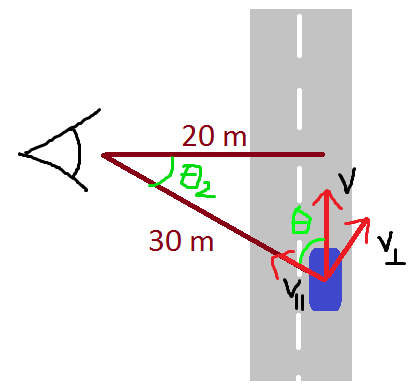
\includegraphics[width=0.5\textwidth]{Astrofysik/Astrofig/PolitiLoesning.png}
		%\caption{Et typisk } %https://upload.wikimedia.org/wikipedia/commons/9/98/Andromeda_Galaxy_%28with_h-alpha%29.jpg
	\end{figure}
	\opg Den radielle hastighed er den parallele komponent med synsvinklen. Vi ser en retvinklet trekant og bruger
	\begin{align}
		cos(\theta)=\frac{\text{hosliggende katete}}{\text{hypotenusen}}=\frac{v_{radiel}}{v} \\
		v_{radiel}=v cos(\theta)
	\end{align}
	Der dannes også en retvinklet trekant af vejen, afstanden til vejen og afstanden til bilen. I grader giver det en vinkel på
	\begin{align}
		cos(\theta_2)&=\frac{20}{30}\\
		\theta_2 &= cos^{-1} \left( \frac{20}{30} \right) = 48
	\end{align}
	De to vinkler indgår begge i en retvinklet trekant, så
	\begin{align}
		180 &= \theta + \theta_2 + 90\\
		\theta &= 90 - \theta_2  = 42
	\end{align}
	Vi indsætter og får
	\begin{align}
	v_{radiel}=50 km/t * cos(42) = 50 km/t * 0.74 = 37 km/t
	\end{align}
	Hvis du ikke får det samme, så prøv at regne alt i radianer, da det er simplere.
	\opg 
	Du står stille, så $v_{obs}=0$. $v_{kilde}$ er den radielle hastighed, som lige skal omregnes til km/t:
	\begin{align}
	37 km/t = 37 \frac{10^{3}m}{60*60 s} = \frac{37}{3.6} m/s = 10,3 m/s
	\end{align}
	Så indsætter vi i
	\begin{align}
	f_{obs} = \frac{340 m/s + 0}{340 m/s - 10,3} 800 Hz = 825 Hz
	\end{align}
	Bemærk hastigheden er negativ i forhold til observatøren.
\end{opgave}
\begin{opgave}{Galaksen M87 i Virgohoben}{1}
	\opg Hubble loven giver, under antagelse af at M87 bevæger sig væk fra jorden som følge af universets udvidelse, at
	\begin{align*}
	v = H_0D
	\end{align*}
	Idet $z<<1$ kan den ikke relativistiske approksimation benyttes
	\begin{align*}
	z\approx\frac{v}{c}
	\end{align*}
	Komineres de to ligninger fås
	\begin{align*}
	D_\text{M87} = \frac{zc}{H_0} = \SI{18,7}{\mega\parsec}
	\end{align*}
	\opg Under antagelse af at strålingen er udsendt isotropt fra M87, så den samlede luminositet
	\begin{align*}
	L_\text{M87} = 4\pi D_\text{M87}^2\cdot f_\text{M87}
	\end{align*}
	Estimatet for antallet af stjerner i M87, $N_\text{M87}$, bliver så
	\begin{align*}
	N_\text{M87} = \frac{L_\text{M87}}{L_\odot} = \SI{4,01e10}{}
	\end{align*}
\end{opgave}
\begin{opgave}{Afstandsbedømmelse i nabolaget}{1}
	\opg Vi ved at
	\begin{align*}
	m-M = 5\log \left( \frac{d_L}{\si{pc}} \right) -5
	\end{align*}
	Og vi vil gerne bestemme $d_L$, så den isoleres. 
	\begin{align*}
	\frac{m-M+5}{5} &= \log \left( \frac{d_L}{\si{pc}} \right) \\
	\Rightarrow 10^{\frac{m-M+5}{5}} &= 10^{\log \left( \frac{d_L}{\si{pc}} \right)}\\
	&= \frac{d_L}{\si{pc}}\\
	\Rightarrow d_L &= 10^{\frac{m-M+5}{5}}\\
	& \approx 56754~\si{pc}
	\end{align*}
	\opg Hvis udslukningen er 60$\%$ vil kun 40 $\%$ af lyset nå os. Det betyder også at 
	\begin{align*}
	0,40f_{faktisk} &= f_{obs}\\
	f_{faktisk} &= \frac{f_{obs}}{0,40}
	\end{align*}
	Vi har nu udtrykket 
	\begin{align*}
	m_1-m_2 = -2,5 \log \left( \frac{f_1}{f_2} \right) 
	\end{align*}	 
	Hvor $f_1$ erstattes med med $f_{faktisk}$. 
	\begin{align*}
	m_{faktisk}-m_{obs} = -2,5 \log \left( \frac{f_{obs}}{0,40f_{obs}} \right) 
	\end{align*}
	Det betyder
	\begin{align*}
	m_{faktisk} &=-2,5\log \left( \frac{1}{0,40} \right) +m_{obs} \\
	&= 16,5
	\end{align*}
	En mindre magnitude betyder, at stjernen lyser klarere. \\
	Så for at bestemme den faktisk afstand indsættes den faktiske tilsyneladende magnitude i udtrykket fra delopgave 1. 
	\begin{align*}
	d_{faktisk} = 35809~\si{pc}
	\end{align*}
\end{opgave} 
\begin{opgave}{Afstande}{1}
	\opg Isolér $D_M$ i hvert udtryk.
	\begin{align}
		D_M &= \frac{D_L}{1+z}\\
		D_M &= D_A(1+z)
	\end{align}
	Resultaterne sættes lig hinanden
		\begin{align}
		\frac{D_L}{1+z} &= D_A(1+z)\\
		D_L &= D_A (1+z)^2
		\end{align}
	\opg Ved $z=1$ er $D_C\approx3200 Mpc$ og derfor
	\begin{align}
		D_L &= D_M(1+z)= 3200 Mpc \cdot 2 = 6400 Mpc\\
		D_A &= \frac{D_M}{1+z}= 3200 Mpc/ 2 = 1600 Mpc.
	\end{align}
	Ved $z=9$ er $D_C\approx9200 Mpc$, så
	\begin{align}
		D_L &= D_M(1+z)= 9200 Mpc \cdot 10 = 92000 Mpc\\
		D_A &= \frac{D_M}{1+z}= 9200 Mpc/ 10 = 920 Mpc.
	\end{align}
	Gamle objekter, der har bevæget sig fra os længere tid, har altså en større luminositetsafstand, men en lavere vinkelafstand ved høje rødforskydninger. Man skulle ellers tro objekter så mindre ud på himlen, jo længere væk de var, hvilket er rigtigt indtil omkring $z=1,6$. I det tidlige univers var galakserne tættere på hinanden, så de fyldte meget på himlen for hinanden, og derfor er deres lys spredt ud over et stort område.
	\opg
	%Dengang var universet for resten kun 250 mio. år gammelt.\\
	Hvis vi approksimerer $z\approx\frac{v}{c}$, får vi overlyshastigheder, så det går ikke.
	\begin{align}
	z+1&=\sqrt{\frac{1+\frac{v}{c}}{1-\frac{v}{c}}}\\
	(z+1)^2&=\frac{1+\frac{v}{c}}{1-\frac{v}{c}}
	\end{align}
	så vi skal løse et system på formen $y=\frac{1+x}{1-x}$, hvor $y=(z+1)^2$ og $x=\frac{v}{c}$. Man kan omformulere det til $x=\frac{y-1}{y+1}$. Derfor må
	\begin{align}
	\frac{v}{c}&=\frac{(z+1)^2-1}{(z+1)^2+1}\\
	v&=\frac{(z+1)^2-1}{(z+1)^2+1} c = \frac{(10+1)^2-1}{(10+1)^2+1} = 0,98 c. %3\cdot 10^{8} m/s =
	\end{align}
	Så svaret er 98 \% af lysets fart i vakuum.
\end{opgave}
\begin{opgave}{Himmellegemers overfladetemperatur}{3}
	\opg For at kunne komme frem til udtrykket starter vi med at se på fluxen, altså det lys, som vi modtager. Fluxen er givet ved
	\begin{align*}
	f &= \frac{L_\odot}{4\pi d^2}\\
	&= \frac{4\pi R_\odot^2 \sigma T_\odot^4}{4\pi d^2}\\
	&= \left( \frac{R_\odot}{d}\right) ^2 \sigma T_\odot^4
	\end{align*}
	Vi ser nu på den energi som planeten absorberer. Vi antager at vi har en jævn kugle, som energien fordeles jævnt udover. Derudover skal vi have albedoen i spil, i det den fortæller os hvor meget lys, der bliver reflekteret. 
	\begin{align*}
	L_\text{abs} &= \pi R_{m}^2 f \left( 1-A\right) \\
	&= \pi R_{m}^2 \left( \frac{R_\odot}{d}\right) ^2 \sigma T_\odot^4 \left( 1-A\right)\\
	&= \frac{\pi R_m^2R_\odot^2 \sigma T_\odot^4}{d^2} \left( 1-A\right) 
	\end{align*}
	\opg I det Solen er en stjerne i termisk ligevægt, det betyder at der bliver udsendt lige så meget energi som der bliver absorberet. 
	\begin{align*}
	L_\text{uds} = 4\pi R_m^2 \sigma T_m^4
	\end{align*}
	\begin{align*}
	L_\text{uds} &= L_\text{abs} \\
	\Rightarrow 4\pi R_m^2 \sigma T_m^4 &= \frac{\pi R_m^2R_\odot^2 \sigma T_\odot^4}{d^2} \left( 1-A\right) \\
	\Rightarrow 4T_m^4 &= \left( \frac{R_\odot}{d} \right) ^2 T_\odot^4 \left( 1-A\right) \\
	\Rightarrow T_m^4 &= \left( \frac{R_\odot}{d} \right) ^2 \frac{\left( 1-A\right)}{4} T_\odot^4\\ 
	\Rightarrow T_m &= \left( \frac{R_\odot}{d} \right) ^{\frac{1}{2}} \left( \frac{\left( 1-A \right) }{4} \right) ^{\frac{1}{4}} T_\odot
	\end{align*}
	\opg Vi bruger udtrykket, som vi lige har fundet og bestemmer temperaturen på overfladen. 
	\begin{align*}
	T_m \approx \SI{40}{\kelvin}
	\end{align*}
	\opg Vi antager at Mimas roterer hurtigt. Det har den betydning, at vi antager at temperaturen er den samme på over det hele, der vil altså ikke være noget ''dag og nat''. Den teoretiske værdi er bestemt til \SI{40}{\kelvin} og temperaturen er blevet vurderet til \SI{65}{\kelvin}. Det tyder derfor på, at vores antagelse om hurtigt rotation muligvis ikke er så god. Hvis den roterer langsomt, vil det betyde at temperaturen ikke er den samme overalt, hvilket kan forklare hvorfor temperaturen er blevet vurderet til \SI{65}{\kelvin}. 
\end{opgave}
\begin{opgave}{Skalafaktor}{2}
	\opg Vi omskriver formlen og indsætter temperaturerne
		\begin{align}
		a(t)=\frac{T_0}{T(t)}\\
		a(t)=\frac{2.73 K}{3000 K} \approx 10^{-3}
		\end{align}
		Så kan denne formel bruges:
		\begin{align}
		a(t) = \frac{1}{1+z}\\
		z = \frac{1}{a(t)} - 1\\
		z = \frac{1}{10^{-3}} - 1 \approx 10^3
		\end{align}
		Så rekombinationen skete ved $z\approx 1000$.
\end{opgave}
\begin{opgave}{Fladt univers med stof}{2}
	\opg Hvis universet er fladt, er $\Omega_{total}=1$. Består det kun af stof, må $\Omega_m=1$ og resten er 0.
	\opg Skalafaktoren er
	\begin{align}
	a(t)=\left(\frac{t}{t_0}\right)^{2/(3+3\omega)} = \left(\frac{t}{t_0}\right)^{2/3}
	\end{align}
	da $\omega=0$ for stof.
	\opg En $10^6.$-del af 1 er $10^{-6}$. Baseret på $z=\frac{a(t_0)}{a(t)}-1$ kan ændring i rødforskydning opskrives
	\begin{align}
		\Delta z =|\frac{a(t_0)}{a(t_0)} - \frac{a(t_0)}{a(t_1)}|= |1-\frac{1}{a(t_1)}|\\
		%\Delta z &= |1-\frac{1}{a(t_1)}|
		 %\sqrt{\frac{1+\frac{\Delta v}{c}}{1-\frac{\Delta v}{c}}} - 1
	\end{align}
	hvor vi sætter $a(t_0)=1$ og $t_1$ er tidspunktet, vi stopper med at observere. Det ligger efter $t_0$, så $|1-\frac{1}{a(t_1)}|=1 - \frac{1}{a(t_1)}$
	Vi isolerer $a(t_1)$ 
	\begin{align}
	a(t_1) = \frac{1}{1-\Delta z} &= \left(\frac{t_1}{t_0}\right)^{2/3} \\
	\frac{t_1}{t_0} &= \left( \frac{1}{1-\Delta z} \right)^{3/2}
	%t_1 &= \left( \frac{1}{\Delta z + 2} \right)^{3/2} t_0
	\end{align}
	Vi indsætter ændringen i $z$
		\begin{align}
		\frac{t_1}{t_0} &= \left( \frac{1}{1-10^{-6}} \right)^{3/2} = 1.0000015
		%t_1 &= \left( \frac{1}{\Delta z + 2} \right)^{3/2} t_0
		\end{align}
	Så vi skal vente til tidspunktet $t_1 = t_0 + \Delta t = 1.0000015*t_0$, hvor $t_0$ er universets nuværende alder.
	\begin{align}
		\Delta t = (1.0000015 - 1) t_0 = 0.0000015 t_0 = 0.0000015*13.8*10^{9} \text{år} - = 20700 \text{år}
	\end{align}
\end{opgave}
\begin{opgave}{Kosmologiske parametre}{0}
	\opg 
	\begin{align}
	H^2=\frac{8\pi G \rho}{3}-\frac{\kappa c^2}{a^2}+\frac{\Lambda}{3}.
	\end{align}
	bliver til
	\begin{align}
	H^2=\frac{8\pi G}{3} (\rho_R+\rho_m+\rho_\Lambda)-\frac{\kappa c^2}{a^2} 
	\end{align}
	Så bruger vi $\rho_R=\rho_{R,0}a(t)^{-4}, \rho_m=\rho_{m,0}a(t)^{-3}$ og $\rho_\Lambda=\rho_{\Lambda,0}$ :
	\begin{align}
	H^2=\frac{8\pi G}{3} (\frac{\rho_{R,0}}{a(t)^4}+\frac{\rho_{m,0}}{a(t)^3}+\rho_\Lambda)-\frac{\kappa c^2}{a^2} 
	\end{align}
	\opg
	Bidraget fra stråling skal være lige så stort som det for stof
	\begin{align}
	\rho_R &= \rho_m\\
	\frac{\rho_{R,0}}{a(t)^4} &= \frac{\rho_{m,0}}{a(t)^3}\\
	\rho_{m,0} a(t) &= \rho_{R,0}\\
	a(t) &= \frac{\rho_{R,0}}{\rho_{m,0}} = 0.000267
	\end{align}
	Så bruger vi
	\begin{align}
		a(t)=\left(\frac{t}{t_0}\right)^{2/(3+3\omega)} = \left(\frac{t}{t_0}\right)^{1/2}\\
		t = a(t)^2 t_0 = 0.000267^2 \cdot 13.8\cdot10^9 \text{år} = 982 \text{år}
	\end{align}
	\opg Det giver noget ca. 50 gange for lavt, da det er en dårlig approksimation at antage universets størrelse udvikler sig som om det består af stråling. Stof og mørk energi har enorm betydning for universets alder $t_0$.
	\opg Mængden af kosmologisk konstant er konstant.
	\begin{align}
		\rho_\Lambda = \Omega_\Lambda \rho_c = 0.6911 \cdot 8.6\cdot 10^{-27} kg/m^3 = 5.9 \cdot 10^{-27} kg/m^3
	\end{align}
	\iffalse % Udkommentering
	Vi kender for stof og stråling
	\begin{align}
		\rho = \rho_0 a^{-3(1+\omega)}
	\end{align}
	 og indsætter $a(t)=\left(\frac{t}{t_0}\right)^{2/(3+3\omega)}$
	 \begin{align}
	 \rho = \rho_0 \left(\left(\frac{t}{t_0}\right)^{2/(3+3\omega)}\right)^{-3(1+\omega)} = \rho_0 \left(\frac{t}{t_0}\right)^{-6(1+\omega)/(3+3\omega)}
	 = \rho_0 \left(\frac{t}{t_0}\right)^{-2} \propto t^{-2}.
	 \end{align}
	 For kosmologisk konstant
	 	\begin{align}
		 	\rho = \rho_0 a^0 = \rho_0 % = \rho_0 e^{H_0(t-t_0)} \propto e^{H_0t}
	 	\end{align}
	 \opg Hvis vi ignorerer kosmologisk konstant, leder vi efter tidspunktet hvor $\Omega_R = 0,9$ og $\Omega_R = 0,1$. Vi husker $\Omega_R=\frac{\rho_R}{\rho_c}$, så vi søger tidspunktet hvor
	 \begin{align}
	 	\rho_R &= \Omega_R \rho_c = 0,9 \cdot 8,6 \cdot 10^{-27}kg/m3 = 7.74 \cdot  10^{-27}kg/m3\\
	 	\rho_m &= \Omega_m \rho_c = 0,1 \cdot 8,6 \cdot 10^{-27}kg/m3 = 0.86 \cdot  10^{-27}kg/m3.
	 \end{align}
	 Vi kender de nuværende værdier, så tidspunktet kan findes ved
	 \begin{align}
	 	t=(\rho_R/\rho_{R,0})^{-1/2} = (\rho_m/\rho_{m,0})^{-1/2}\\
	 	=(\Omega_R/\Omega_{R,0})^{-1/2} = (\Omega_m/\Omega_{m,0})^{-1/2}
	 	=
	 \end{align}
	 %Nej, regn a først, det her giver 2 forskellige ting
	 \fi
\end{opgave}
\begin{opgave}{Andromeda-galaksen}{2}
	\opg Ligning 1.22 i kompendiet giver at
	\begin{align*}
	v^2 = \frac{GM(R)}{R}
	\end{align*}
	Her isoleres $M(R)$ som er massen af af den del af Andromeda-galaksen, som ligger indenfor afstanden $R$ fra centrum, og de opgivne værdier indsættes
	\begin{align*}
	M(R) = \frac{v^2R}{G} = \SI{2,45e42}{\kilo\gram} = \SI{1,23e12}{M_\odot}
	\end{align*}
	\opg 
	\begin{align}
	D_H=\frac{v}{H_0} 
	\end{align}
	Vi skal bruge den radielle hastighed
	\begin{align}
	v \approx z c = -0.001 \cdot 3\cdot 10^8 m/s =-3\cdot 10^5 m/s
	\end{align}
	og omskriver Hubble-konstanten en lille smule
	\begin{align}
	H_0=70 km s^{-1} Mpc^{-1} = 7 \cdot 10^4 m s^{-1} Mpc^{-1}.
	\end{align}
	Vi indsætter
	\begin{align}
	D_H=\frac{-3\cdot 10^5 m s^{-1}} {7 \cdot 10^4 m s^{-1} Mpc^{-1}} = - 3/7 \cdot 10 Mpc = - 4,2 Mpc.
	\end{align}
	Så Hubble-afstanden bryder sammen og giver noget negativt.
	\opg Vi omregner lysår til meter
	\begin{align}
	2.5\cdot 10^6 \text{lysår} = 2.5\cdot 10^6 \cdot 9,46 \cdot 10^15 m = 23.7 \cdot 10^21 m\\
	\frac{23.7 \cdot 10^21 m}{3\cdot 10^5 m/s} = 7.9 \cdot 10^16 s = 2,5 \cdot 10^9 \text{år}
	\end{align} 
	Så det vil tage 2,5 mia. år, hvis vi ser bort fra accelerationen og andre effekter. I virkeligheden er det 4-5 mia. år.
	Stjernerne er ligger meget spredt i begge galakser, så vi kommer ikke til at støde ind i andre. Når gassen fra galakserne kolliderer varmes det op og vi vil se en masse ny stjernedannelse. Galakserne vil med tiden smelte sammen til en elliptisk galakse, der har opbrugt det meste gas, så der ikke dannes flere stjerner. 
\end{opgave}

\begin{opgave}{Betelgeuse}{1}
	\opg Hvis vi antager at Betelgeuse er et sfærisk sortlegeme, der udsender sortlegemestråling kan vi beregne dens luminositet vha. formel (1.25) fra kompendiet
	\begin{align*}
	L_\odot &= 4\pi R_\odot^2\sigma T_\odot^4 =\SI{3.839e26}{\watt} \\
	L_B &= 4\pi R_B^2\sigma T_B^4 =\SI{5,886e31}{\watt} = \SI{1,533e5}{L_\odot}
	\end{align*}
	\opg Fluxen fra et isotropt udstrålende stortlegeme er ved negligering af ekstinktion
	\begin{align*}
	f_B = \frac{L_B}{4\pi d_B^2} = \SI{1,27e-7}{\watt\per\metre\squared}
	\end{align*}
	\opg Fluxen fra solen på jorden, $L_\odot$ er, under samme antagelser som før, givet som
	\begin{align*}
	f_\odot = \frac{L_\odot}{4\pi d_\odot^2}
	\end{align*}
	hvorfor
	\begin{align*}
	f_\odot = f \quad&\Rightarrow\quad \frac{L_\odot}{4\pi d_\odot^2} = \frac{L_B}{4\pi d^2} \\
	\Rightarrow\quad d &= \sqrt{\frac{L_B}{L_\odot}d_\odot} = \SI{392}{AU}
	\end{align*}
	\opg Idet $d\approx2.8\cdot d_V$ ville man skulle næsten 3 gange længere væk fra Betelgeuse end Voyager 1 er fra Solen, hvilket er en afstand meget større end solsystemes radius, da Voyager 1 er omkring udkanten af solsystemet. Afstanden er dog ikke sammenlignelige med den til Proxima Centauri, fordi $d$ ca. er 1.4\permil af $d_{PC}$.
\end{opgave}
\begin{opgave}{Massen af Solsystemet}{1}
	\opg Idet Neptuns bane er antaget cirkulær er den tilbagelagte afstand, $D$, iløbet af én periode
	\begin{align*}
	D = 2\pi R
	\end{align*}
	hvorved den gennemsnitlige banefart bliver
	\begin{align*}
	v = \frac{d}{P} = \frac{2\pi R}{P} = \SI{5,42}{\kilo\metre\per\second}
	\end{align*}
	\opg For himmelegemer i cirkulære baner er
	\begin{align*}
	v^2 = \frac{GM(R)}{R}
	\end{align*}
	hvorved massen af solsystemet approksimeres til
	\begin{align*}
	M(R) = \frac{Rv^2}{G} = \frac{4\pi^2R^3}{GP^2} = \SI{0,994}{M_\odot}
	\end{align*}
\end{opgave}